  \textbf{\subsection{Определение числа каскадов}}
  \vspace{1em}

\subsubsection{Номинальный сквозной коэффициент передачи:}
	
\begin{equation}
  \label{eq:equation1_1}
  K_{\text{Е}} = \dfrac{U_{\text{н}}}{E_{\text{г}}} = \dfrac{\sqrt{P_{\text{н}} R_{\text{н}} }}{E_{\text{г}}}
\end{equation}


\begin{equation*}
  K_{\text{Е}} =  \dfrac{\sqrt{8 \cdot 2 }}{0.045} = 88.889
\end{equation*}
  
  \subsubsection{Запас усиления для обеспечения заданных характеристик усилителя:}
  
  1) Запас на введение ООС, численно равный глубине обратной связи:
  
\begin{equation}
  \label{eq:equation1_2}
  F \geq \dfrac{K_{\text{г ок}}}{K_{\text{г}}}
\end{equation}

\begin{equation*}
  F \geq \dfrac{0.15}{0.01} = 15.0
\end{equation*}

\noindent где $ K_{\text{г ок}} = 15 \ldots 20 \% $ -- коэффициент гармоник оконечного двухтактного каскада без ООС.\par

 2) Запас на регулировку тембра, определяемый коррекцией частотной характеристика:
 
 \begin{equation}
  \label{eq:equation1_3}
  m \geq 10^{ \left| \Delta b_{\text{т}}  
   \right| /20 }
\end{equation}

\begin{equation*}
  m \geq 10^{ \left| \pm 14.0  \right| /20 } = 5.012
\end{equation*}

3) Технический запас, учитывающий разброс параметров компонентов:
 
\begin{equation*}
  K_{\text{з}} = 1,5 \ldots 2 
\end{equation*}
  
\subsubsection{Требуемый сквозной коэффициент усиления:}

\begin{equation}
  \label{eq:equation1_4}
  K_{\text{Е тр}} \geq K_{\text{Е}} \cdot F \cdot m \cdot K_{\text{з}}
\end{equation}

\begin{equation*}
  K_{\text{Е тр}} \geq 88,889 \cdot 14 \cdot 5,012 \cdot 2 \geq 13364,9
\end{equation*}
    
\subsubsection{Определяем число каскадов усиления по напряжению}


\begin{equation}
  \label{eq:equation1_5}
  n \geq \dfrac{\lg(K_{\text{Е тр}})}{\lg(K_n)}
\end{equation}

\noindent где $ K_n = 30 \ldots 40 $ -- усредненный коэффициент усиления по напряжению для одного каскада.\par	

 \begin{equation*}
   n \geq \dfrac{\lg( 13364,9 )}{\lg( 35 )} \geq 2,67 \approx 3
\end{equation*} 

\subsubsection{Входное сопротивление каскада предварительного усилителя:}


\begin{equation}
  \label{eq:equation1_6}
  R_{\text{вх}} \geq (5 \ldots 10) R_{\text{г}}
\end{equation}
\begin{equation*}
   R_{\text{вх}} \geq 7 \cdot 10\cdot 10^3 = 70 ~\text{кОм}
\end{equation*}   

В связи с величиной  Rвх на входе усилителя желательно включить дополнительный согласующих  каскад по схеме с общем истоком. \par 
На рис.~\ref{figure:p1_2} РУ~--~регулятор усиления; СК~--~согласующий каскад; КПУ~--~каскад предварительного усиления; РТ~--~регулятор тембра; ВК~--~входной каскад усилителя мощности (УМ); ПОК~--~предоконечный каскад УМ; ОК~--~оконечный каскад УМ; ООС~--~цепь обратной связи УМ; БП~--~блок питания; ФП~--~фильтр питания.
\clearpage
\begin{figure}[htbp]
    \center{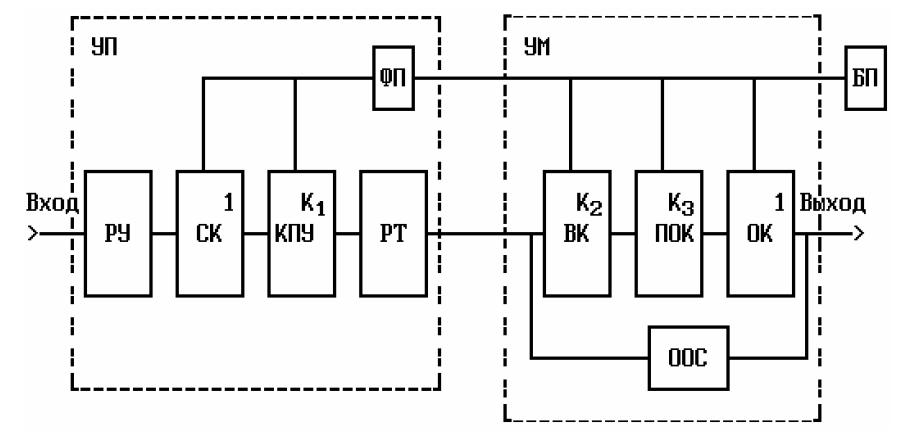
\includegraphics[width=0.8\linewidth]{picture_2}}
    \caption{Структурная схема усилителя сигналов звуковой частоты}
    \label{figure:p1_2}
  \end{figure}
  
  
